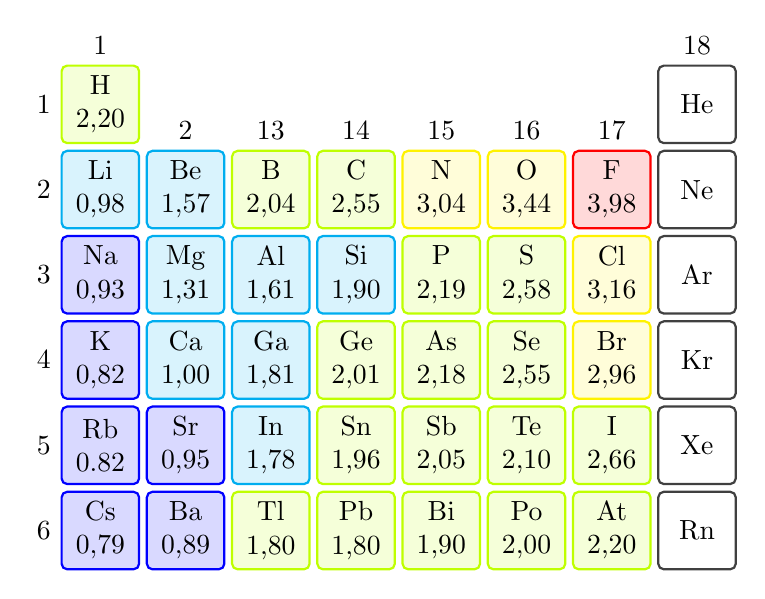
\begin{tikzpicture}
  \def\sep{2pt} % Node distance
  \tikzset
    {
      element/.style = 
        {
          rectangle,
          rounded corners = 2pt,
          thick,
          fill = #1!15,
          draw = #1,
          minimum size = 2.8em,
          align = center,
        },
      n-element/.style = 
        {
          rectangle,
          rounded corners = 2pt,
          thick,
          draw = black!75,
          minimum size = 2.8em,
        },
    }  
  % GRUPO 1
  \node (Li) [element = cyan] 
    { \ce{Li} \\ \num{0,98} };
  \node (Na) [element = blue, anchor = north, yshift = -\sep] at (Li.south) 
    { \ce{Na} \\ \num{0,93} };
  \node (K) [element = blue, anchor = north, yshift = -\sep] at (Na.south) 
    { \ce{K} \\ \num{0,82} };
  \node (Rb) [element = blue, anchor = north, yshift = -\sep] at (K.south) 
    { \ce{Rb} \\ \num{0.82} };
  \node (Cs) [element = blue, anchor = north, yshift = -\sep] at (Rb.south) 
    { \ce{Cs} \\ \num{0,79} };

  % GRUPO 2
  \node (Be) [element = cyan, anchor = west, xshift = \sep] at (Li.east) 
    { \ce{Be} \\ \num{1,57} };
  \node (Mg) [element = cyan, anchor = north, yshift = -\sep] at (Be.south) 
    { \ce{Mg} \\ \num{1,31} };
  \node (Ca) [element = cyan, anchor = north, yshift = -\sep] at (Mg.south) 
    { \ce{Ca} \\ \num{1,00} };
  \node (Sr) [element = blue, anchor = north, yshift = -\sep] at (Ca.south) 
    { \ce{Sr} \\ \num{0,95} };
  \node (Ba) [element = blue, anchor = north, yshift = -\sep] at (Sr.south) 
    { \ce{Ba} \\ \num{0,89} };

  % GRUPO 13
  \node (B) [element = lime, anchor = west, xshift = \sep] at (Be.east) 
    { \ce{B} \\ \num{2,04} };
  \node (Al) [element = cyan, anchor = north, yshift = -\sep] at (B.south) 
    { \ce{Al} \\ \num{1,61} };
  \node (Ga) [element = cyan, anchor = north, yshift = -\sep] at (Al.south) 
    { \ce{Ga} \\ \num{1,81} };
  \node (In) [element = cyan, anchor = north, yshift = -\sep] at (Ga.south) 
    { \ce{In} \\ \num{1,78} };
  \node (Tl) [element = lime, anchor = north, yshift = -\sep] at (In.south) 
    { \ce{Tl} \\ \num{1,80} };

  % GRUPO 14
  \node (C) [element = lime, anchor = west, xshift = \sep] at (B.east) 
    { \ce{C} \\ \num{2,55} };
  \node (Si) [element = cyan, anchor = north, yshift = -\sep] at (C.south) 
    { \ce{Si} \\ \num{1,90} };
  \node (Ge) [element = lime, anchor = north, yshift = -\sep] at (Si.south) 
    { \ce{Ge} \\ \num{2,01} };
  \node (Sn) [element = lime, anchor = north, yshift = -\sep] at (Ge.south) 
    { \ce{Sn} \\ \num{1,96} };
  \node (Pb) [element = lime, anchor = north, yshift = -\sep] at (Sn.south) 
    { \ce{Pb} \\ \num{1,80} };

  % GRUPO 15
  \node (N) [element = yellow, anchor = west, xshift = \sep] at (C.east) 
    { \ce{N} \\ \num{3,04} };
  \node (P) [element = lime, anchor = north, yshift = -\sep] at (N.south) 
    { \ce{P} \\ \num{2,19} };
  \node (As) [element = lime, anchor = north, yshift = -\sep] at (P.south) 
    { \ce{As} \\ \num{2,18} };
  \node (Sb) [element = lime, anchor = north, yshift = -\sep] at (As.south) 
    { \ce{Sb} \\ \num{2,05} };
  \node (Bi) [element = lime, anchor = north, yshift = -\sep] at (Sb.south) 
    { \ce{Bi} \\ \num{1,90} };

  % GRUPO 16
  \node (O) [element = yellow, anchor = west, xshift = \sep] at (N.east) 
    { \ce{O} \\ \num{3,44} };
  \node (S) [element = lime, anchor = north, yshift = -\sep] at (O.south) 
    { \ce{S} \\ \num{2,58} };
  \node (Se) [element = lime, anchor = north, yshift = -\sep] at (S.south) 
    { \ce{Se} \\ \num{2,55} };
  \node (Te) [element = lime, anchor = north, yshift = -\sep] at (Se.south) 
    { \ce{Te} \\ \num{2,10} };
  \node (Po) [element = lime, anchor = north, yshift = -\sep] at (Te.south) 
    { \ce{Po} \\ \num{2,00} };

  % GRUPO 17
  \node (F) [element = red, anchor = west, xshift = \sep] at (O.east) 
    { \ce{F} \\ \num{3,98} };
  \node (Cl) [element = yellow, anchor = north, yshift = -\sep] at (F.south) 
    { \ce{Cl} \\ \num{3,16} };
  \node (Br) [element = yellow, anchor = north, yshift = -\sep] at (Cl.south) 
    { \ce{Br} \\ \num{2,96} };
  \node (I) [element = lime, anchor = north, yshift = -\sep] at (Br.south) 
    { \ce{I} \\ \num{2,66} };
  \node (At) [element = lime, anchor = north, yshift = -\sep] at (I.south) 
    { \ce{At} \\ \num{2,20} };

  % GRUPO 18
  \node (Ne) [n-element, anchor = west, xshift = \sep] at (F.east) 
    { \ce{Ne} };
  \node (Ar) [n-element, anchor = north, yshift = -\sep] at (Ne.south) 
    { \ce{Ar} };
  \node (Kr) [n-element, anchor = north, yshift = -\sep] at (Ar.south) 
    { \ce{Kr} };
  \node (Xe) [n-element, anchor = north, yshift = -\sep] at (Kr.south) 
    { \ce{Xe} };
  \node (Rn) [n-element, anchor = north, yshift = -\sep] at (Xe.south) 
    { \ce{Rn} };

  % PRIMEIRO PERÍODO
  \node (H) [element = lime, anchor = south, yshift = \sep] at (Li.north) 
    { \ce{H} \\ \num{2,20} };
  \node (He) [n-element = red, anchor = south, yshift = \sep] at (Ne.north) 
    { \ce{He} };

  % LABELS GRUPO
  \node [anchor = south] at (H.north)  {1};
  \node [anchor = south] at (Be.north) {2};
  \node [anchor = south] at (B.north)  {13};
  \node [anchor = south] at (C.north)  {14};
  \node [anchor = south] at (N.north)  {15};
  \node [anchor = south] at (O.north)  {16};
  \node [anchor = south] at (F.north)  {17};
  \node [anchor = south] at (He.north) {18};

  % LABELS PERÍODO
  \node [anchor = east] at (H.west)  {1};
  \node [anchor = east] at (Li.west) {2};
  \node [anchor = east] at (Na.west) {3};
  \node [anchor = east] at (K.west)  {4};
  \node [anchor = east] at (Rb.west) {5};
  \node [anchor = east] at (Cs.west) {6};
  
\end{tikzpicture}

